\section{计数性质与指标定义}
\paragraph{事件身份。}
每次物理请求和执行事件具有唯一身份。新增事件集合为 $N$ 时，增量工作为 $\Delta\W=\sum_{e\in N}\mathbf w(e)$。重复读取同一日志只计算一次；实际重试产生新的事件身份，再次计入。导入前缀保留历史消耗并将新增消耗置零，因此完整路径满足 $\W_{0\rightarrow u}=\W_0+\Delta\W_u$。

\paragraph{单位不变性。}
对坐标 $j$ 使用正数 $a_j$ 改变单位，同时乘两个方案的对应坐标，不改变支配不等式，也不改变 $1-a_jW_j(\ell)/(a_jW_j(h))$。这解释了为何可以保留异质原生单位，不必加权成总分。不同资源的代价偏好仍由使用场景决定。

\paragraph{时间可加关系。}
模型与工人活动并集满足容斥关系 $|I_M\cup I_W|=U_M+U_W-O$。从经过时间减去活动并集得到其他开销。并行工人时长之和不作为墙钟时间。原生回放采用 $|I_W|$，在线采用运行开始至完成的经过时间；验证和证据重执行另记账。

\paragraph{数据库工作代理。}
SQLite 每 1,000 条虚拟机指令触发一次进度处理器。历史字段名为 \nolinkurl{sqlite_vm_steps_lower_bound}，本文以回调数或其乘 1,000 的值作为工作代理。短查询可以为零，准备阶段及数据库版本也会影响回调行为，因此不将其写成精确指令数。A14 的 19.5 倍是 39/2 次回调之比。

\paragraph{指标分工。}
五场景主要工作量坐标依次为图论文记录读取数、原生回归用例数、SQLite 进度工作代理、指标值读取数和业务记录读取数。其余原生坐标仍全部进入支配判断。主要坐标分母为零时不计算节省比例，底表保留绝对值。
交付率为已提交并评分阶段数除以计划阶段数。$Q_1$ 检查输出契约，$Q_2$ 检查证据和状态，$\G$ 为二者合取。工作量为事件求和向量，支配关系保留资源取舍。$S_W,S_T,D$ 比较指定计时域中的工作和收益。$A_{\rm rel},A_{\rm irr}$ 测量有效前缀后的修复和保持。增量工作、模型请求、时间与费用说明更新代价。前缀审计区分答案变化、证据刷新和可复用状态。

\section{来源和改造细节}
\paragraph{图数据。}
STaRK 冻结版本为 \nolinkurl{88269e23e90587f99476c5dd74e235a0877e69be}。原切片有 16,550 个节点和 149,765 条边；Stanford、MIT、Tokyo 切片分别有 16,058/142,401、14,376/126,927、13,167/120,386 个节点/边。扩展过程在指定机构中按种子抽取作者，保留发表记录和外向引用。焦点作者与原集合不重叠，引用节点有重叠。四簇分配 8/4/4/4 个父任务。

\paragraph{代码数据。}
Requests 固定在 \nolinkurl{b25c87d7cb8d6a18a37fa12442b5f883f9e41741}，ItsDangerous 固定在 \nolinkurl{096c8d42545d3b68ea21a4f890fb2b2d8979c0bd}。packaging 和 python-dotenv 使用发布的 25.0 与 1.1.1 源码包，并记录 SHA-256。四簇分别分配 4/4/6/6 个父任务。原始、植入和修复快照独立保存，公开预期与当前观察分离。用例绑定包、检查名、用例名和版本；有效结论要求精确指出范围内失败项。

\paragraph{关系数据。}
BIRD debit 与 financial 各四个父任务，Chinook 与 Northwind 各六个。消费任务聚合指定年份和客户；贷款任务聚合地区与状态；采购任务统计去重订单数、行数量和行金额，Northwind 应用折扣。相关变化改变对象集或受控数据值。原生汇总函数与等价只读 SQL 都可以通过验证。

\paragraph{遥测数据。}
RCAEval 扩展文件固定版本为 \nolinkurl{afeacb11bcc94dadfd1c8f483ee4377b2b8b614e}。原 checkout 簇八个父任务，currency CPU、product-catalog delay 和 Train Ticket order CPU 各四个。保留指标、日志、链路和注入时间。公开切分点及过滤条件确定期望量，相关卡片只移动切分点。任务评价源遥测派生的诊断报告。

\paragraph{应用数据。}
四份 AppWorld 导出来自 \nolinkurl{b0a8eae_1}、\nolinkurl{22cc237_1}、\nolinkurl{3fcc458_1}、\nolinkurl{90adc3f_1}，父任务分配为 4/4/6/6。后两份分别包含六/四个播放列表、32/43 个支付请求和各 106 条用户记录。适配器在导出记录上实现本地状态变化：播放允许任一满足时长的列表，下载保持既有集合，支付按成员身份替换为 $\max(0,\mathrm{share}-\mathrm{paid})$。验证器检查最终状态。

\section{模型配置与验收}
全部模型通过 OpenRouter 调用，记录 provider、量化信息及请求参数。六个端点按开源模型家族归组，四个归为闭源 API；Qwen3.8 Flash 是日志中的生产端点，未绑定到某个公开检查点。最终新增 Grok 4.3、MiniMax M3、Gemini 3.7 Flash、GPT-6 Luna、GLM-5.3 Flash。Mistral Small 4 在正式阶段开始前持续限流，由 GLM 替换。

开发阶段冻结 JSON 对象和推理设置：GLM、Gemini 3.7、Luna 使用低推理，Grok 和 MiniMax 关闭推理。早期模型使用记录的兼容配置。全体保持相同原生工人和任务预算。在线配对匹配采集组及准入段，GLM 延后采集单列一组。原生回放在共同批次执行，Python 为 3.13.4，SQLite 为 3.49.1。

任务层验收通过 784 项，扩展契约验收通过 19 项，等价证据验收通过 11 项。非对象答案保护使 20 个畸形例子均被拒绝，并保留正常评分分支。等价性审计恢复两个 MiniMax 有效阶段，不改变模型响应及轨迹。四条传输错误占位记录不算模型 JSON 格式错误，仍保留于物理台账。

新增五模型有 3,000 个逻辑阶段、3,008 个物理阶段尝试；2,994 个逻辑阶段提交并评分，六个没有提交。四个物理请求保留未知费用预约。质量、交付和传输状态独立保存；最终 6,000 个逻辑阶段全部具有终态记录。

\section{补充结果与分母}
\begin{table*}[t]
\centering\small\setlength{\tabcolsep}{5pt}
\begin{tabular}{lrrrrrr}
\toprule
Model & Submitted & $Q_1$ & $\G$ & Initial $\G$ & Related $\G$ & Irrelevant $\G$ \\
\midrule
DeepSeek V4 Pro 0813 & 600/600 & 295/600 & 269/600 & 117/200 & 9/117 & 117/117 \\
Kimi K2.6 & 596/600 & 397/600 & 374/600 & 153/200 & 52/153 & 152/153 \\
Qwen3.8 Flash & 575/600 & 410/600 & 402/600 & 159/200 & 72/159 & 152/159 \\
Gemma 4 31B & 571/600 & 458/600 & 406/600 & 161/200 & 81/161 & 161/161 \\
GLM-5.3 Flash & 600/600 & 550/600 & 526/600 & 184/200 & 150/184 & 182/184 \\
MiniMax M3 & 600/600 & 97/600 & 52/600 & 19/200 & 0/19 & 19/19 \\
Gemini 3.8 Flash & 599/600 & 531/600 & 530/600 & 196/200 & 135/196 & 196/196 \\
Gemini 3.7 Flash & 600/600 & 537/600 & 534/600 & 197/200 & 140/197 & 197/197 \\
Grok 4.3 & 594/600 & 270/600 & 221/600 & 97/200 & 3/97 & 96/97 \\
GPT-6 Luna & 600/600 & 563/600 & 559/600 & 196/200 & 165/196 & 196/196 \\
\bottomrule\end{tabular}
\caption{精确分母。Submitted 表示已提交并评分；最后两列以初始有效为条件，因此不是相应 200 个更新阶段的无条件有效数。}
\label{tab:zh_counts}\end{table*}
\begin{figure*}[t]
\centering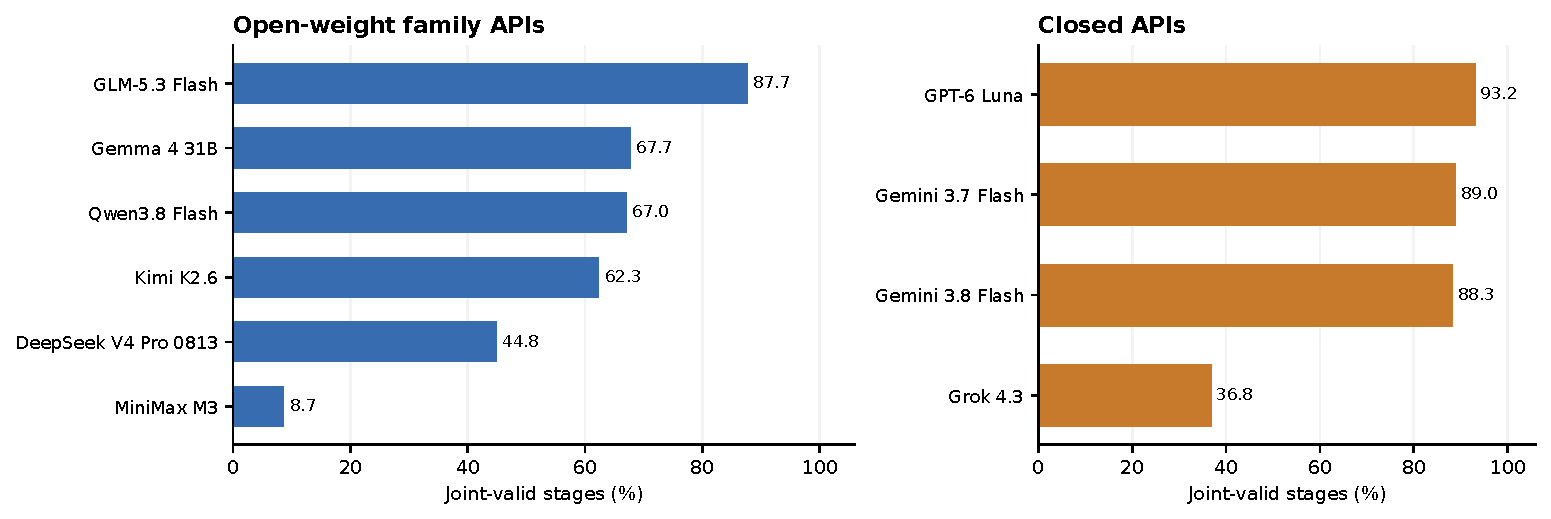
\includegraphics[width=.96\textwidth]{figure_5_validity.pdf}
\caption{按端点家族分组的描述性质量排行。分数为 600 个阶段的有效率；不合并工作量、时间及适应指标。}
\end{figure*}

初始、相关和无关条件的无条件有效数分别为 1,479、862、1,532，分母均为 2,000。条件更新比较中，相关与无关有效数分别为 807、1,468，分母为 1,479。差异来自无条件更新还包含初始无效状态的继续执行。

中等任务一工人回放中，121/467 对正向衰减，14/467 对无正收益，332/467 对至少等比例兑现，父任务等权差距为 $-7.9$ 个百分点，区间 $[-15.6,1.0]$。四工人相应为 108、27、332 对，平均差距 $-6.0$ 个百分点。

相同 116 对方案中，四工人原生节省比在线节省高 41.3 个百分点，区间 24.4--61.1；去掉本地准入后为 24.2 个百分点，区间 13.9--34.5。统计先在父任务内部平均，再在 37 个父任务间平均。

来源感知适应分析先在父任务内平均有效重复，再做场景内来源簇和父任务重采样。Luna 的相关更新父任务等权估计为 83.3\%，区间 76.7--89.7；GLM 为 81.1\%，区间 74.0--87.7。这与按有效重复数直接合并略有不同。全部十模型共同通过的初始交集仅八个父任务--重复单元，因此另提供每对模型的共同支持集。

\section{相关工作覆盖映射}
\begin{table*}[t]
\centering\small
\setlength{\tabcolsep}{3pt}
\begin{tabular}{lccccc}
\toprule
Evaluation & Executed outcome & Native work vector & Work--time pairing & Relevant updates & Valid-prefix cost\\
\midrule
WorFBench & $\circ$ & -- & -- & -- & --\\
FlowBench / FlowMind & $\checkmark$ & -- & -- & -- & --\\
AgentBoard & $\checkmark$ & -- & -- & -- & --\\
AppWorld & $\checkmark$ & -- & -- & -- & --\\
ClawArena-Team & $\checkmark$ & -- & -- & $\checkmark$ & --\\
OrchBench & $\circ$ & $\circ$ & $\circ$ & -- & --\\
\textbf{WELD} & $\checkmark$ & $\checkmark$ & $\checkmark$ & $\checkmark$ & $\checkmark$\\
\bottomrule
\end{tabular}
\caption{按本文操作定义映射的已报告测量。勾选为直接覆盖，圆圈为相关但测量域不同，横线为未单独报告该协议。Native work vector 保留领域单位；Work--time pairing 配对比较有效方案的原生工作与实际时间；Valid-prefix cost 测量有效完成前缀后的新增代价。}
\label{tab:zh_coverage}
\end{table*}

WorFBench v3 以结构匹配为主，并报告下游执行及计时；FlowMind v1 评价执行与重建工作流，包含 token 和工具分析；AgentBoard 报告进度和过程分析；AppWorld 通过应用状态检验结果。ClawArena-Team v2 具有执行评分、分阶段变化、权限及模态指标和使用量分析。OrchBench v1 通过确定性模拟测量质量、工期和 token。矩阵按照本文操作定义映射，对模拟域或粒度不同的量标记部分覆盖。最后一列要求从已验证完成前缀测量新增成本，并有相关/无关对照。

\section{复现材料}
底表包含 6,000 个阶段、5,006 对初始比较、各工作坐标、计时资格、前缀审计、适应比较池与来源敏感性分析。绘图代码直接使用这些表。完整研究归档索引初始计划、修订、观察、物理尝试及不可变源快照。任务卡和验证器代码独立保留。正文采用最终审计数值，开发探针和早期极复杂先导实验单独归档。
